\chapter{Initial data set collection: Insights and experiences}
\label{chap:results}

\section{A Simple Approach to Data Set Acquisition}
With the current setup, the threshold for recording high-quality data sets is very low.
Following is the comprehensive list of steps required to start the \sr and record video.
\begin{enumerate}
    \item Connect the battery to the \jx.
    \item Enable mobile hotspot on your phone with name and password set to\textit{sensorrig}.
    \item Wait for the \sr to connect and find its IP address under hotspot settings.
    \item Go to \textit{http://<ip-address>:8080} in a web browser.
    \item Start the recording in the \textit{Run} tab.
    \item Start the \gls{ptp} deamons in the \gls{ptp} tab.
    \item Collect your dataset and monitor the video in the \textit{Video} tab.
\end{enumerate}
This simplie workflow takes only a couple minutes and enables effortless usage of the \sr, as it requires minimal training or technical expertise.
It is anticipated that this user-friendly setup will encourage widespread utilization of the \sr by both myself and other researchers and master's students at NTNU in the future.


\section{Polarization Data}
\label{sec:pol_benefits}
The \sr is capable of reliably capturing 10-bit polarization video at a frame rate of 16fps.
These images contain four distinct polarization channels, as illustrated in Figure \ref{fig:stacked_pols}.
This presents a valuable advantage in maritime environments, where reflected light exhibits polarization characteristics, as evidenced by the varying intensities observed in the four channels.

\begin{figure}[H]
    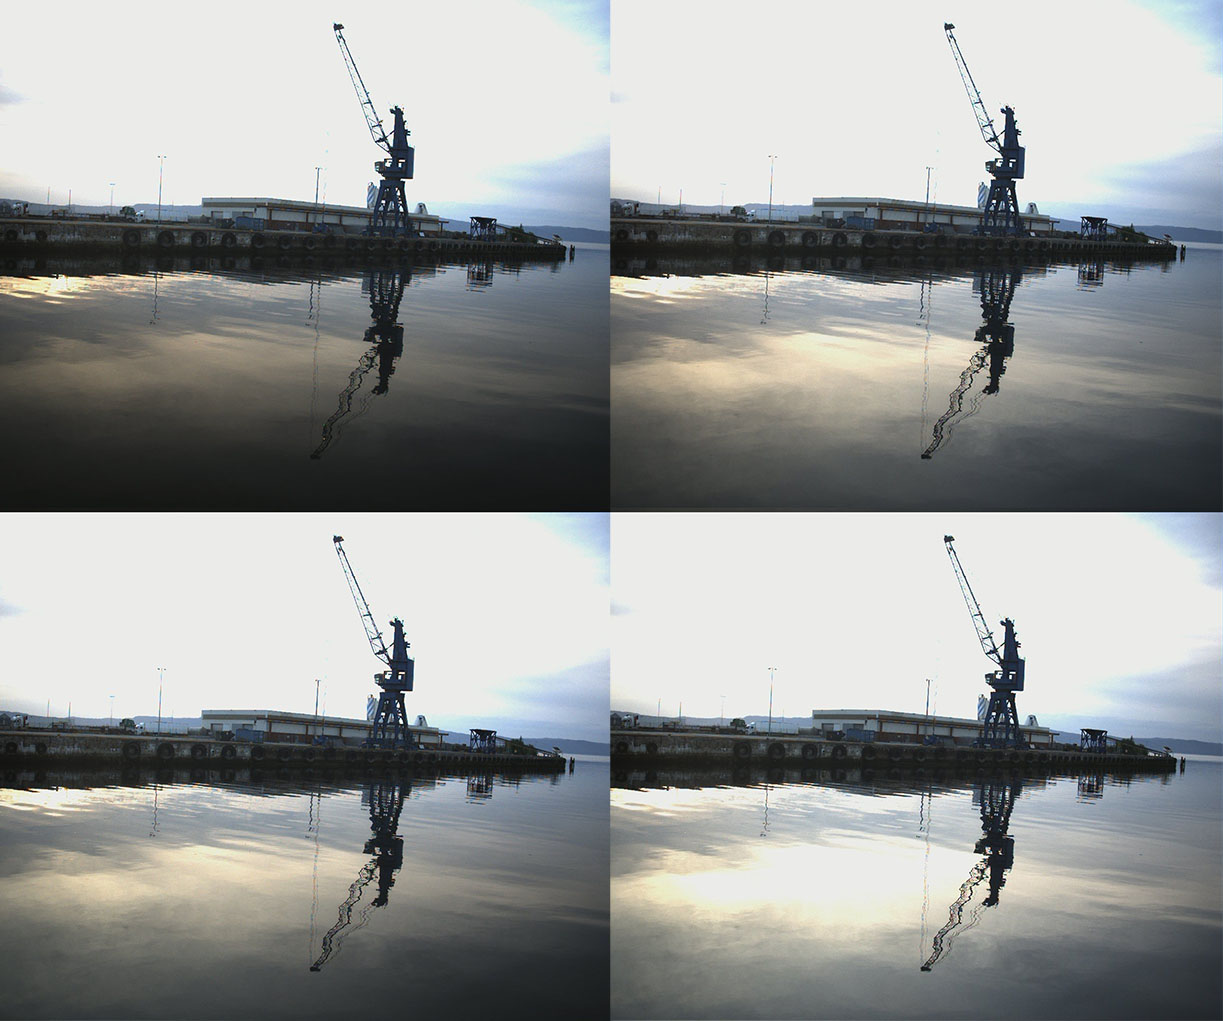
\includegraphics[width=\textwidth]{figures/pictures/stacked_right_148.jpg}
    \caption{The four polarization channels with $0^\circ$, $45^\circ$, $90^\circ$ and $135^\circ$ polarization angle respectiverly.}
    \label{fig:stacked_pols}
\end{figure}


To facilitate visualization, a simple toolkit was developed, employing the Equation \todo to calculate \gls{dolp} and \gls{aolp} from the four polarization channels.
These values can be visualized as hue and value in the \gls{hsv} color space.
The application of this visualization is demonstrated in the image below (Figure \ref{fig:picture_1536}).

The image clearly showcases the potential benefits of polarization imaging in maritime environments, as the water is distinctly visible.
However, there are several issues that deserve attention.
Five regions of interest are marked in the image and will be discussed in the following sections.

\begin{figure}[H]
    \centering
    \subcaptionbox{Avraged image.
        Simliar to "normal" camera.
        \label{fig:normal_img_1536}}{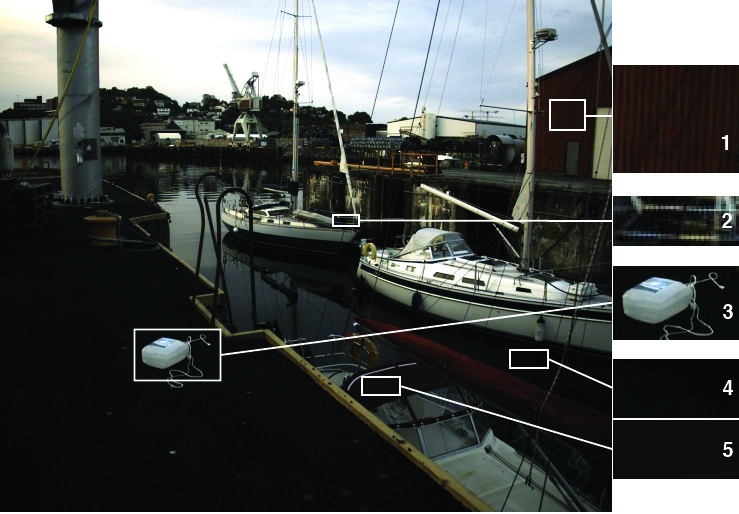
\includegraphics[width=\textwidth]{figures/pictures/result_rgb-80.jpg}}
    \subcaptionbox{\gls{aolp} and \gls{dolp} visualized as hue and value.
        \label{fig:pol_img_1536}}{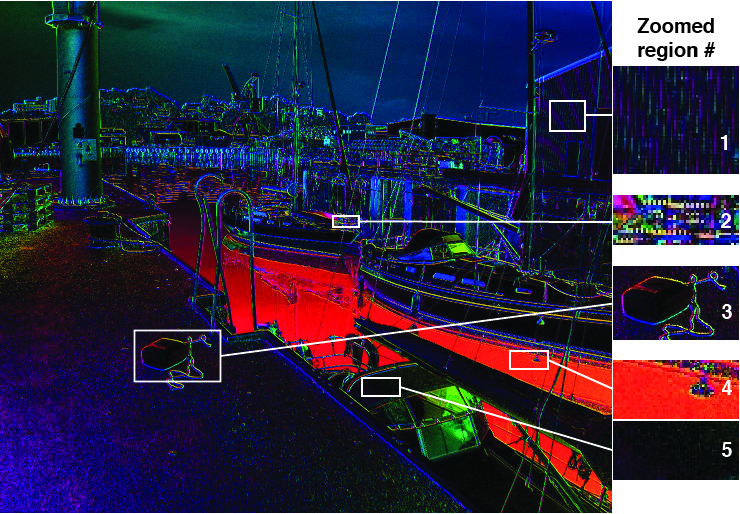
\includegraphics[width=\textwidth]{figures/pictures/result_pol-80.jpg}}
    \caption{Right image \#1536 with, zoomed in regions of interest.}
    \label{fig:picture_1536}
\end{figure}

\subsection{Region 3: Artificial Polarization fom Gradients}
\label{sec:artifical_polarization}

Region 3 exhibits what appears to be artificial polarization.
These artifacts are likely caused by high image gradients.
As the four polarization angles are spatially separated in the \gls{pfa} this gradient results in different intnsities in the four polarization channels even though the light is unpolarized.
Consequently, the estimation of the polarization may be incorrect in such cases.

Various papers have been published on polarization estimation techniques for both monochrome and color polarization cameras \cite{mihoubiSurveyDemosaickingMethods2018} \cite{spoteJointDemosaicingColour2021}.
However, none of these methods were compatible with the current setup.
Nevertheless, they can serve as sources of inspiration for future work in this area.

Section \ref{sec:better_analysation_tools} delves into the potential implementation of improved analysis tools in future endeavors.

\subsection{Region 1: Aliasing}
As each polarization group (\gls{pg}) is formed by combining four pixels, the spatial separation between each \gls{cg} is greater compared to a regular camera.
Consequently, effects such as aliasing are expected to be more pronounced in the captured images.

This phenomenon can be observed in region 1 of Figure \ref{fig:picture_1536}, where the aliasing is visible.
The polarization analysis of this area also reveals the presence of aliasing effects in the polarization domain.
It is believed that these aliasing effects in the polarization domain are caused by the artificial polarization discussed in Section \ref{sec:artifical_polarization}.


\subsection{Region 2: Zipper Effect and False Colors}

In addition to aliasing, zipper effect and false colors are also observed in high-frequency regions.
This can be seen in region 2 of Figure \ref{fig:normal_img_1536} and is further amplified in the polarization image.
There are noticeable color artifacts in the regular image, where a white bar appears slightly blue and then slightly yellow.
These observations suggest that there might be room for improvement in the debayering algorithm to mitigate these issues and achieve better color accuracy.

\subsection{Region 4 and 5: Polarization Reveals Water}
One significant advantage of polarization imaging in maritime environments is that water reflections exhibit polarization.
As a result, it becomes relatively straightforward to detect water in the image by analyzing the differences in polarization, as depicted by the contrast between region 4 and 5 in Figure \ref{fig:pol_img_1536}.
However, it should be noted that this effect becomes weaker further away as the angle of incidence deviates further away from the Brewster's angle.


\section{Wide Baseline Stereo Data}
The \sr is believed to be the first platform offering offering stereo polarization imaging.
With a baseline of up to $1m$ depth can be estimated further away than off the shelf stereo cameras like the ZED camera.
Beyond the refular benefits of stereo imaging, it is believed that this setup can be used to further enhance depth perception.
This is because \gls{dolp} and \gls{aolp} can be used to support the point correspondance step of the stereo matching algorithm.
Further, it is believed that having two mearusrements of \gls{aolp} from different viewpoints can be used to estimate a normal map of the surfaces in the scend, which can be used to further enhance the depth estimation.
In Figure \ref{fig:picture_1984_left} and \ref{fig:picture_1984_right} we see a matching pair of images from the \sr.
\begin{figure}[H]
    \centering
    \subcaptionbox{Avraged image.
        Simliar to "normal" camera.}{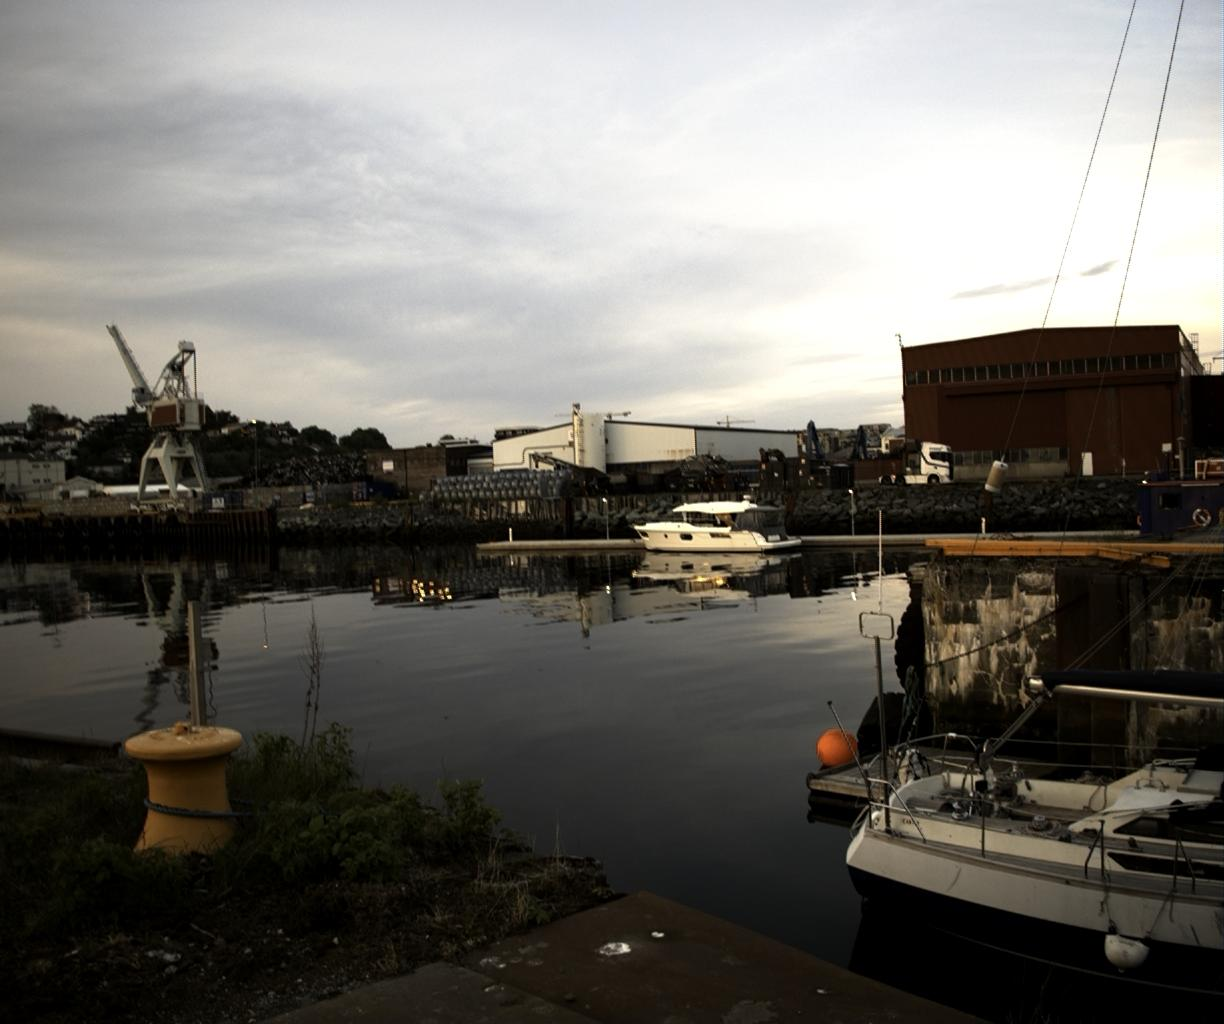
\includegraphics[width=.9\textwidth]{figures/pictures/regular_left_124.jpeg}}
    \subcaptionbox{\gls{aolp} and \gls{dolp} visualized as hue and value.}{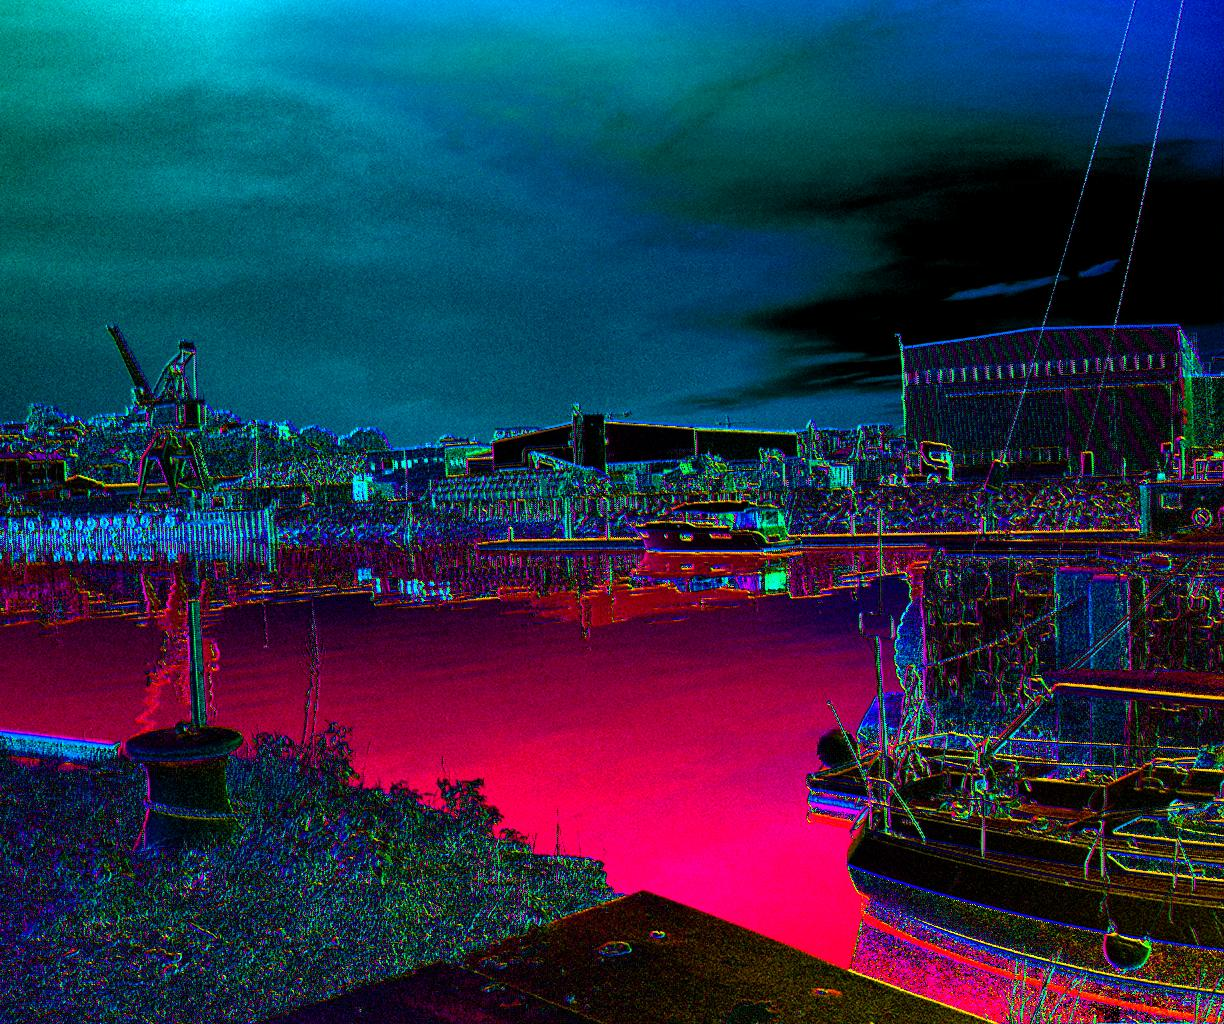
\includegraphics[width=.9\textwidth]{figures/pictures/aolp_left_124.jpeg}}
    \caption{Left image \#1984.
        \label{fig:picture_1984_left}}
\end{figure}
\begin{figure}[H]
    \centering
    \subcaptionbox{Avraged image.
        Simliar to "normal" camera.}{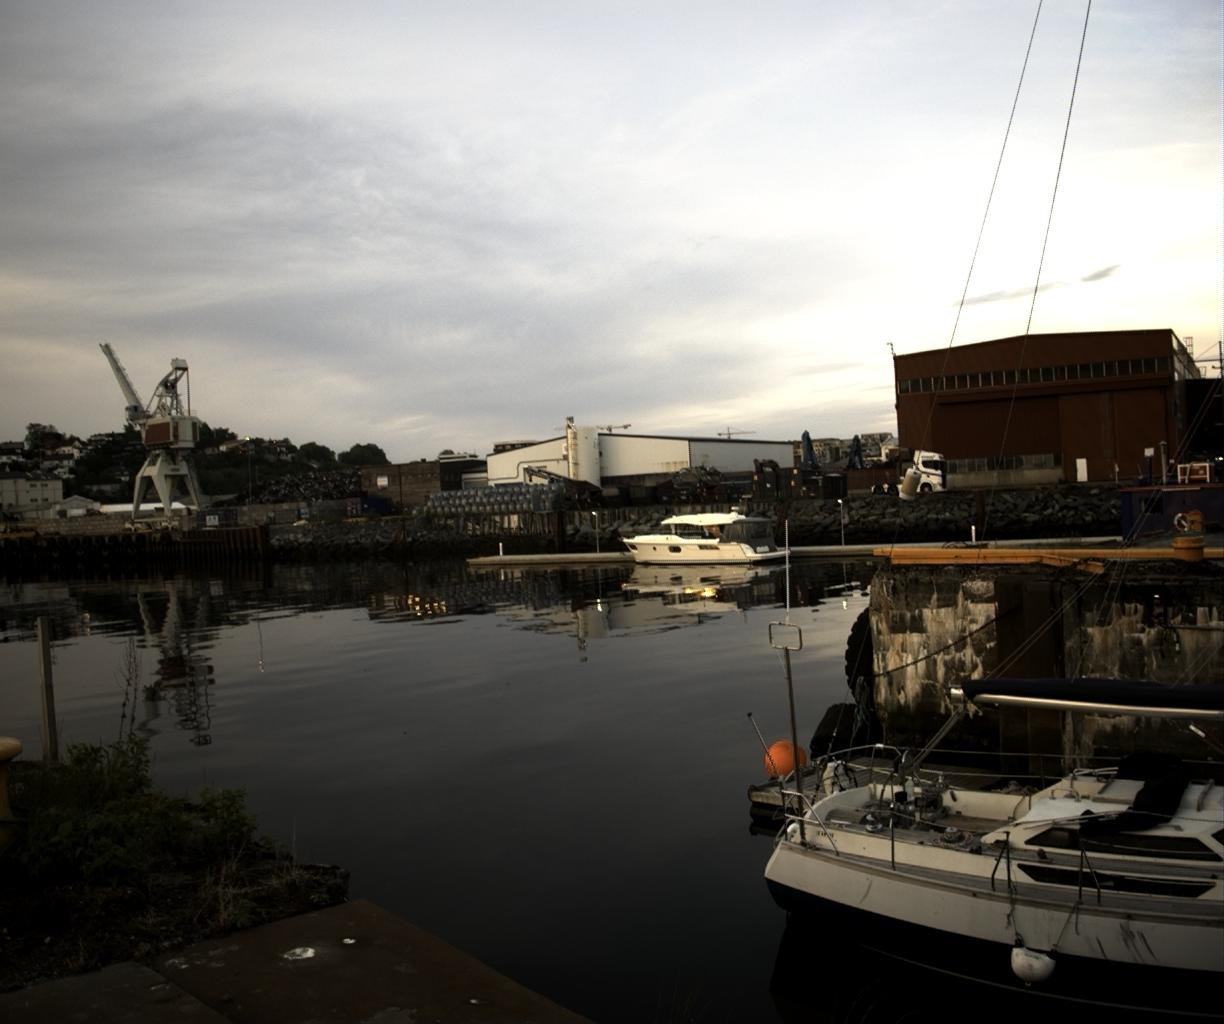
\includegraphics[width=.9\textwidth]{figures/pictures/regular_right_124.jpeg}}
    \subcaptionbox{\gls{aolp} and \gls{dolp} visualized as hue and value.}{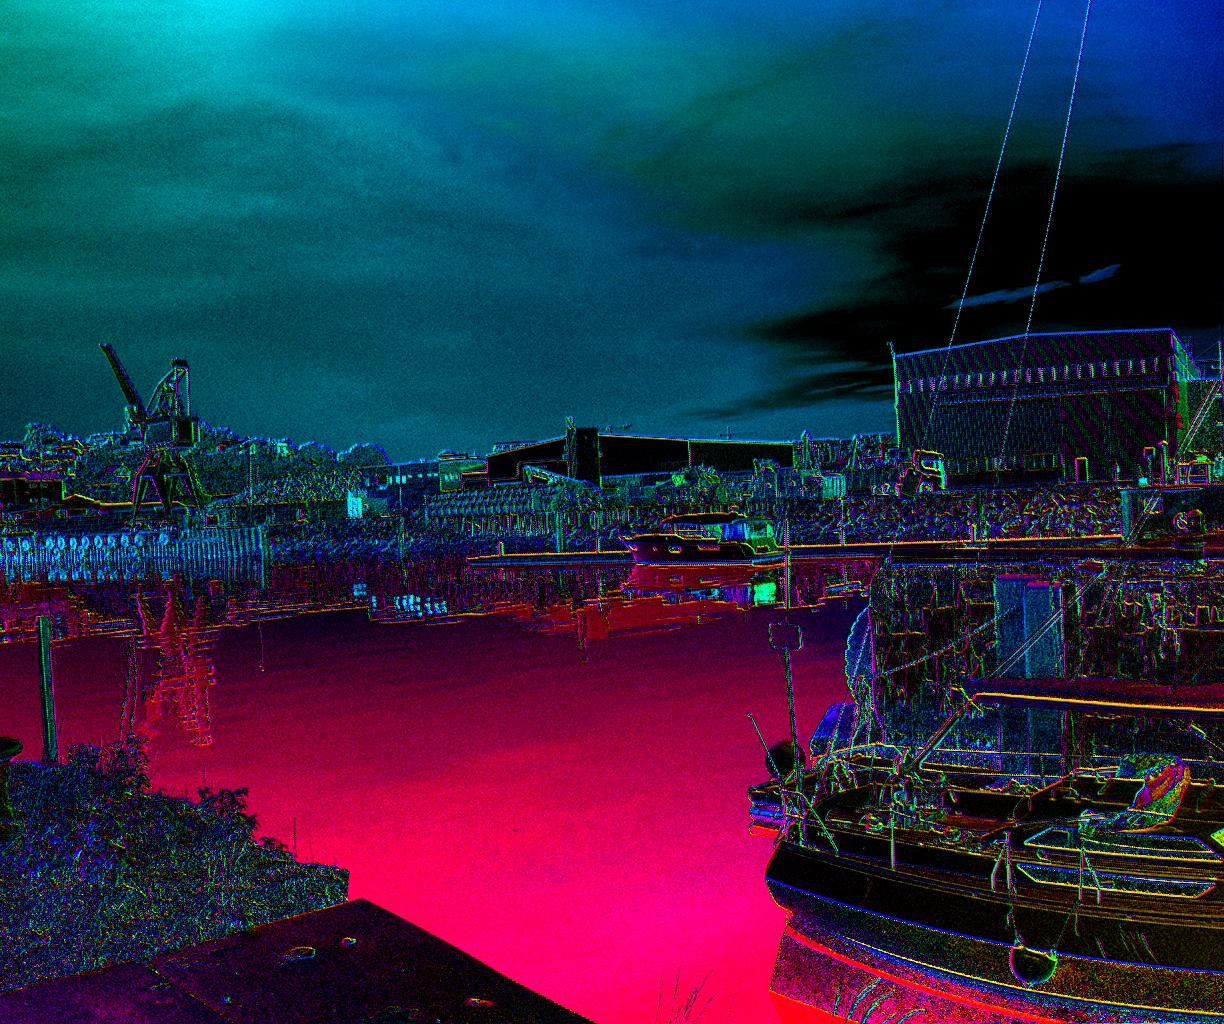
\includegraphics[width=.9\textwidth]{figures/pictures/aolp_right_124.jpeg}}
    \caption{Right image \#1984.
        \label{fig:picture_1984_right}}
    \label{fig:picture_1984}
\end{figure}

\section{10 Bit Images}
Another noteworthy benefit of the final setup is that we get images with 10 bit depth.
This give the images higher dynamic range as the pixel values are more nuanced.
A visualization of this is is shown in Figure \ref{fig:gained_image} where digital gain is applied to the image in Figure \ref{fig:normal_img_1536}, revealing that the darker regions do contain a lot of information.
This probably contributes to why polarization information can be extracted from region 4 in Figure \ref{fig:picture_1536}.

\begin{figure}[H]
    \centering
    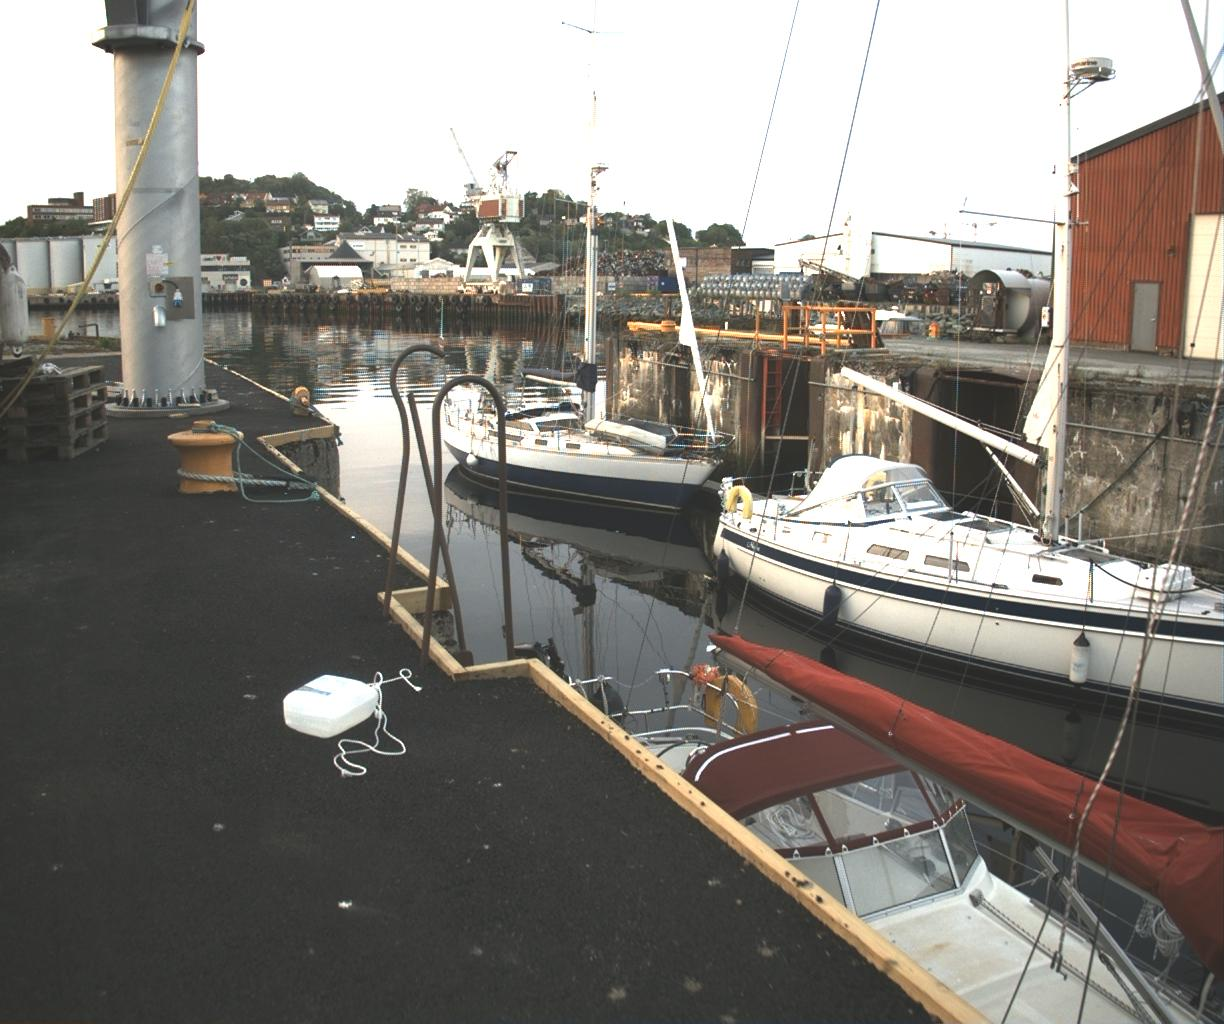
\includegraphics[width=.8\textwidth]{figures/pictures/gained_right_96.jpeg}
    \caption{Image showing how dark areas contain a lot of information thanks to 10-bit depth.
        The image is the same as in Figure \ref{fig:normal_img_1536}, but with digitally increased brightnes.}
    \label{fig:gained_image}
\end{figure}


\section{Highly Efficient Image Preprocessing}

The latency of the preprocessing kernel, discussed in Chapter \ref{chap:debayer}, was measured to be $1.13ms$ using the \code{nsys profile} command line tool from the\gls{cuda} toolkit.
The kernel is launched with only two thread blocks, indicating that we are utilizing a maximum of two out of the eight available \glspl{sm} on the \gls{gpu} \cite{rigerunNVIDIAJetsonXavier2023}.
Considering a frame rate of 2$\times$16 frames per second, this suggests that less than $1\%$ of the \gls{gpu} resources are being utilized for preprocessing.

\begin{equation}
    \frac{2 \times 16 \text{f}/s}{1 \text{f} / 1.13ms} \times \frac{2 \text{SM}}{8 \text{SM}} = 0.904\%
\end{equation}

This estimation aligns with the observation of $0\%$ \gls{gpu} utilization reported by \gls{jtop} for most of the time.
In contrast to the initial implementation using \gls{opencv} on the CPU, where all CPU cores were running at maximum frequency without achieving 32 frames per second, the \gls{gpu} implementation demonstrates a substantial improvement.
This offers advantages such as reduced power consumption and increased availability of both \gls{cpu} and \gls{gpu} resources for other tasks.
These benefits are relevant for potential future works involving real-time experiments.


\section{GStreamer Pipeling with Hardware Accelerated Compression}

The implementation of a \gls{gstreamer} pipeline with hardware-accelerated compression enables longer recording times and the ability to stream compressed images to the graphical user interface and other potential clients.
Having a functional \gls{gstreamer} environment is also crucial for future work, as it allows for the utilization of \gls{gstreamer} and \gls{deepstream} plugins for image processing and analysis.

During the \master, funding was secured to upgrade the \jx to a \jo platform, which has been ordered.
One notable distinction between these platforms is that the \jo supports \gls{av1} encoding in addition to the encoding formats supported by the \jx \cite{karumbunathanNVIDIAJetsonAGX2022}.
Due to the higher efficiency of \gls{av1} compared to \gls{h265}, time was not invested in tuning the compression parameters for \gls{h265} \cite{torresAV1VsHEVC2022}.
Nonetheless, a brief test was conducted to provide a rough estimate of the expected compression performance of the \gls{h265} encoder.

To measure the compression ratio and error, a test video was recorded while walking around the boat yard area at Nyhavna, capturing the same areas depicted in Figures \ref{fig:picture_1984} and \ref{fig:picture_1536}.
Only one camera was enabled during the recording to be able to write the raw data to disk fast enough.
By utilizing the encoding parameters listed in Table \ref{tab:encoder_parameters}, a compression ratio of almost $4/1$ was achieved, with an average relative error less than $0.8\%$ and a maximum relative error below $9\%$.

It is important to note that these encoding parameters were not tuned, and the results may not necessarily be indicative of the performance that can be achieved with \gls{h265}.
Further testing is scheduled as part of the migration to the \jo platform.

\begin{table}[H]
    \begin{minipage}[b]{.5\linewidth}
        \centering
        \small
        \begin{tabular}{|c|c|}
            \hline
            \textbf{Parameter} & \textbf{Value} \\
            \hline
            preset-level       & 0              \\
            ratecontrol-enable & 0              \\
            profile            & Main10         \\
            control-rate       & 0              \\
            maxperf-enable     & 1              \\
            qp-range           & 0,1:0,1:0,1    \\
            \hline
        \end{tabular}
    \end{minipage}
    \begin{minipage}[b]{.5\linewidth}
        \centering
        \small
        \begin{tabular}{|c|c|}
            \hline
            \textbf{Parameter} & \textbf{Value} \\
            \hline
            quant-i-frames     & 0              \\
            quant-p-frames     & 0              \\
            quant-b-frames     & 0              \\
            iframeinterval     & 16             \\
            num-Ref-Frames     & 8              \\
            num-B-Frames       & 1              \\
            \hline
        \end{tabular}
    \end{minipage}
    \caption{Encoder parameters used for testing.}
    \label{tab:encoder_parameters}
\end{table}